\section{Unsupervised Activity Representation}
\subsection{BP-HMM with Orderings (BP-HMM-O)}
\begin{figure}[h!]
  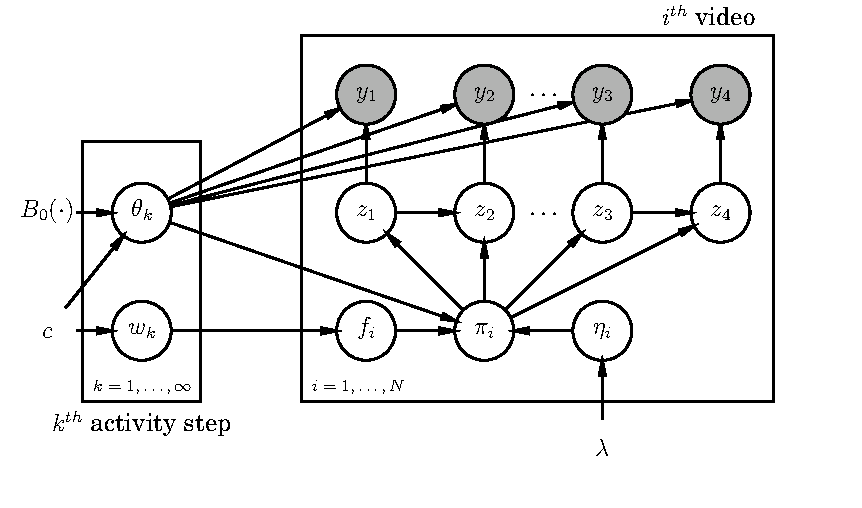
\includegraphics[width=0.5\textwidth]{plate}
  \caption{Graphical model for BP-HMM-O}
  \label{bphmmo}
\end{figure}

\subsection{Gibbs sampling for BP-HMM-O}
Mostly deferred to supplementary, just say we ne need to sample a,b,c,etc. and we used MH for binary and Gibbs for continous/discrete ones.
